% @Author: Taha Bouhsine


%%%%%%%%%%%%%%%%%%%%%%%%%%%%
% CHAPTER                  %
%%%%%%%%%%%%%%%%%%%%%%%%%%%%
\chapter{Tools, Technologies and Languages Used}%
\label{chap:chapter_two}
\section{Mean Stack}
\begin{figure}[!ht]
    \center
    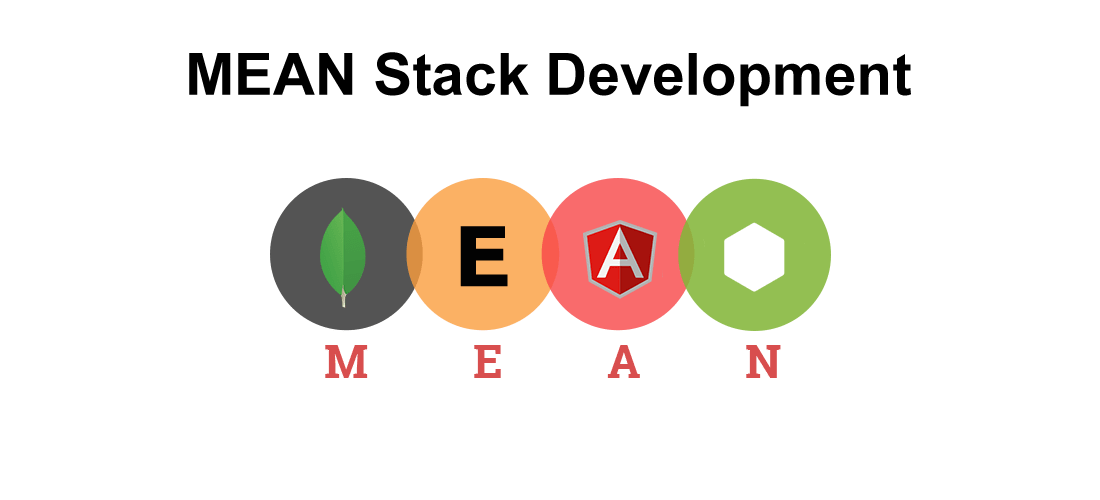
\includegraphics[scale=0.30]{assets/meanstack.png}
\end{figure}

While the name sounds like “mean”, it actually stands for the software pieces that are used to create a particular development stack: MongoDB, ExpressJS, Angular, and NodeJS. One of the biggest advantages of using this particular development stack is the ability to allow developers to use one consistent data model across the stack, using JSON and BSON (for MongoDB). This allows for quick transitions between the various pieces of the stack, especially when a single programmer has to handle more than one portion of the stack.

\begin{figure}[!ht]
    \center
    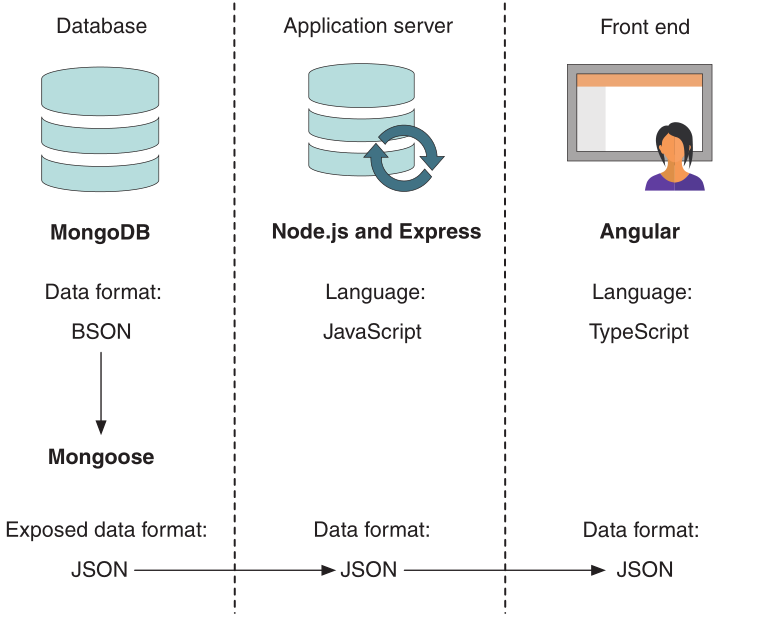
\includegraphics[scale=0.60]{assets/mean.png}
    \caption{Mean Stack}
    \label{fig:mean}
\end{figure}

\section{Model View Controller Design Pattern}

The Model View Controller (MVC) design pattern specifies that an application consist of a data model, presentation information, and control information. The pattern requires that each of these be separated into different objects.

MVC is more of an architectural pattern, but not for complete application. MVC mostly relates to the UI / interaction layer of an application. We’re still going to need business logic layer, maybe some service layer and data access layer.



\begin{enumerate}
    \item Model contains only the pure application data, it contains no logic describing how to present the data to a user.
    \item View presents the model’s data to the user. The view knows how to access the model’s data, but it does not know what this data means or what the user can do to manipulate it.
    \item Controller exists between the view and the model. It listens to events triggered by the view (or another external source) and executes the appropriate reaction to these events. In most cases, the reaction is to call a method on the model. Since the view and the model are connected through a notification mechanism, the result of this action is then automatically reflected in the view.
\end{enumerate}

\begin{figure}[!ht]
    \center
    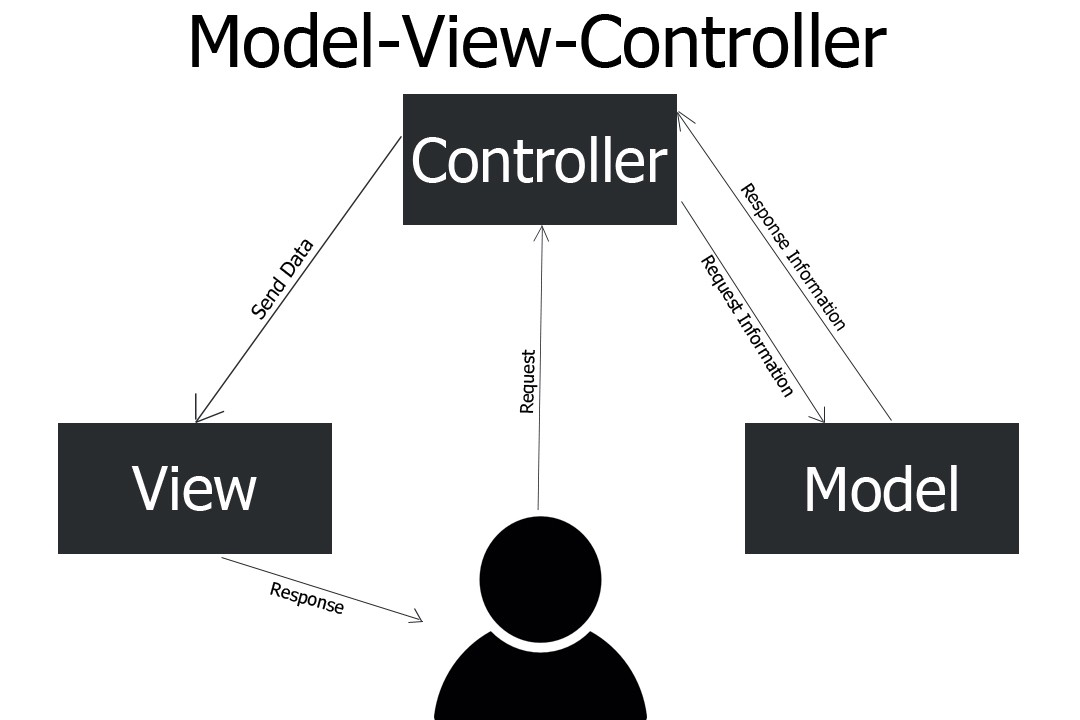
\includegraphics[scale=0.30]{assets/mvc.jpg}
    \caption{Model View Controller}
    \label{fig:mvc}
\end{figure}

\section{Representational State Transfer Architecture}
REST, or REpresentational State Transfer, is an architectural style for providing standards between computer systems on the web, making it easier for systems to communicate with each other. REST-compliant systems, often called RESTful systems, are characterized by how they are stateless and separate the concerns of client and server. We will go into what these terms mean and why they are beneficial characteristics for services on the Web.




\section{Software as a Service}
Software as a Service or SaaS , which allows us to set up services, such as application servers and databases, as needed to create the apps we need. This type of system typically works in a cloud or hybrid cloud environment, which often makes provisioning of servers and software as simple as entering some configurations and clicking a button.

This type of setup is perfect for the MEAN stack, as each piece of the MEAN stack is easily placed into the cloud and thus can be easily provisioned, so they are widely available on SaaS services and can be used quickly when needed. If we are looking for a good development stack, the MEAN stack has much to offer for IT management as well as for developers!



\section{Monolithic Applications}

If all the functionalities of a project exists in a single codebase, then that application is known as monolithic application. We all must have designed a monolithic application in our lives in which we were given a problem statement and were asked to design a system with various functionalities. We design our application in various layers like presentation, service and persistence and then deploy that codebase as single jar/war file. This is nothing but a monolithic application where “mono” represents the single codebase containing all the required functionalities.
\begin{figure}[!ht]
    \center
    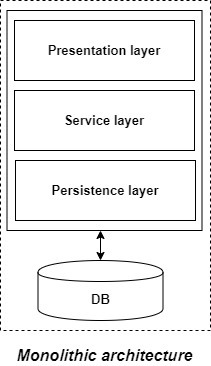
\includegraphics[scale=0.60]{assets/monolithic.jpg}
    \caption{Monolithic Applications}
    \label{fig:monoapp}
\end{figure}

Disadvantages of Monolithic applications:
\begin{enumerate}
    \item
          It becomes too large in size with time and hence, difficult to manage.
    \item
          We need to redeploy the whole application even for a small change.
    \item
          As the size of the application increases, its start-up and deployment time also increases.
    \item
          For any new developer joining the project, it is very difficult to understand the logic of large Monolithic application even if his responsibility is related to a single functionality.
    \item
          Even if a single part of the application is facing a large load/traffic, we need to deploy the instances of the whole application in multiple servers. It is very inefficient and takes up more resources unnecessarily. Hence, horizontal scaling is not feasible in monolithic applications.
    \item
          It is very difficult to adopt any new technology which is well suited for a particular functionality as it affects the whole application, both in terms of time and cost.
    \item
          It is not very reliable as a single bug in any module can bring down the whole monolithic application.
\end{enumerate}
Advantages of monolithic applications:
\begin{enumerate}
    \item
          Simple to develop relative to microservices where skilled developers are required in order to identify and develop the services.
    \item
          Easier to deploy as only a single jar/war file is deployed.
    \item
          Relatively easier and simple to develop in comparison to microservices architecture.
    \item
          The problems of network latency and security are relatively less in comparison to microservices architecture.
\end{enumerate}


\section{Conception}
\subsection{Unified Modeling Language}
\subsection{PlantUml}
PlantUML is an open-source tool allowing users to create UML diagrams from a plain text language. The language of PlantUML is an example of a Domain-specific language. It uses Graphviz software to lay out its diagrams. It has been used to allow blind students to work with UML. PlantUML also helps blind software engineers to design and read UML diagrams.


\subsection{Gantt chart}
A gantt chart is a horizontal bar chart that visually represents a project plan over time. Modern gantt charts typically show us the status of—as well as who’s responsible for—each task in the project.

In other words, a gantt chart is a super-simple way to keep us out of a project pinch!

What are the key parts of a gantt chart?
A gantt chart is made up of several different elements:
\begin{enumerate}
    \item
          Task list: Runs vertically down the left of the gantt chart to describe project work and may be organized into groups and subgroups
    \item
          Timeline: Runs horizontally across the top of the gantt chart and shows months, weeks, days, and years
    \item
          Dateline: A vertical line that highlights the current date on the gantt chart
    \item
          Bars: Horizontal markers on the right side of the gantt chart that represent tasks and show progress, duration, and start and end dates
    \item
          Milestones: Yellow diamonds that call out major events, dates, decisions, and deliverables
    \item
          Dependencies: Light gray lines that connect tasks that need to happen in a certain order
    \item
          Progress: Shows how far along work is and may be indicated by \% Complete and/or bar shading
    \item
          Resource assigned: Indicates the person or team responsible for completing a task
\end{enumerate}


\section{Design}
\subsection{Adobe Photoshop}
Adobe Photoshop is a software application for image editing and photo retouching for use on Windows or MacOS computers. Photoshop offers users the ability to create, enhance, or otherwise edit images, artwork, and illustrations. Changing backgrounds, simulating a real-life painting, or creating an alternative view of the universe are all possible with Adobe Photoshop. It is the most widely used software tool for photo editing, image manipulation, and retouching for numerous image and video file formats. The tools within Photoshop make it possible to edit both individual images as well as large batches of photos.
We used it to prototype and create our platform logo.
\subsection{Adobe XD}
Adobe XD is a vector-based user experience design tool for web apps and mobile apps, developed and published by Adobe Inc. It is available for macOS and Windows, although there are versions for iOS and Android to help preview the result of work directly on mobile devices. XD.


\section{Front-End}
We decided to go with the single page application instead of the multiple pages application and we will be using the following tools for the front end.
\subsection{HTML}
Hypertext Markup Language (HTML) is the standard markup language for documents designed to be displayed in a web browser. It can be assisted by technologies such as Cascading Style Sheets (CSS) and scripting languages such as JavaScript.

Web browsers receive HTML documents from a web server or from local storage and render the documents into multimedia web pages. HTML describes the structure of a web page semantically and originally included cues for the appearance of the document.



\subsection{CSS}
Cascading Style Sheets (CSS) is a style sheet language used for describing the presentation of a document written in a markup language like HTML.[1] CSS is a cornerstone technology of the World Wide Web, alongside HTML and JavaScript.[2]

CSS is designed to enable the separation of presentation and content, including layout, colors, and fonts.[3] This separation can improve content accessibility, provide more flexibility and control in the specification of presentation characteristics, enable multiple web pages to share formatting by specifying the relevant CSS in a separate .css file, and reduce complexity and repetition in the structural content.


\subsection{Typescript}
TypeScript is an open-source programming language developed and maintained by Microsoft. It is a strict syntactical superset of JavaScript and adds optional static typing to the language. TypeScript is designed for development of large applications and transcompiles to JavaScript.[5] As TypeScript is a superset of JavaScript, existing JavaScript programs are also valid TypeScript programs.

TypeScript may be used to develop JavaScript applications for both client-side and server-side execution (as with Node.js or Deno). There are multiple options available for transcompilation. Either the default TypeScript Checker can be used,[6] or the Babel compiler can be invoked to convert TypeScript to JavaScript.

TypeScript supports definition files that can contain type information of existing JavaScript libraries, much like C++ header files can describe the structure of existing object files. This enables other programs to use the values defined in the files as if they were statically typed TypeScript entities. There are third-party header files for popular libraries such as jQuery, MongoDB, and D3.js. TypeScript headers for the Node.js basic modules are also available, allowing development of Node.js programs within TypeScript.

The TypeScript compiler is itself written in TypeScript and compiled to JavaScript. It is licensed under the Apache License 2.0. TypeScript is included as a first-class programming language in Microsoft Visual Studio 2013 Update 2 and later, beside C\# and other Microsoft languages. An official extension allows Visual Studio 2012 to support TypeScript as well. Anders Hejlsberg, lead architect of C\# and creator of Delphi and Turbo Pascal, has worked on the development of TypeScript.



\subsection{Angular 9}
Angular is an app-design framework and development platform for creating efficient and sophisticated single-page apps in html, css, and Typescript which is a superset of JavaScript. Angular provides built-in features for animation, http service, and materials which in turn have features such as auto-complete, navigation, toolbar, menus, etc. The code is written in Typescript, which compiles to JavaScript and displays the same in the browser.
\subsection{Hypertext Transfer Protocol}
The Hypertext Transfer Protocol (HTTP) is an application protocol for distributed, collaborative, hypermedia information systems. HTTP is the foundation of data communication for the World Wide Web, where hypertext documents include hyperlinks to other resources that the user can easily access, for example by a mouse click or by tapping the screen in a web browser.
\subsection{JSON}
JavaScript Object Notation (JSON) is an open standard file format, and data interchange format, that uses human-readable text to store and transmit data objects consisting of attribute–value pairs and array data types (or any other serializable value). It is a very common data format, with a diverse range of applications, such as serving as a replacement for XML in AJAX systems.

JSON is a language-independent data format. It was derived from JavaScript, but many modern programming languages include code to generate and parse JSON-format data. The official Internet media type for JSON is application/json. JSON filenames use the extension .json.



\section{Back-End}
\subsection{Javascript}
JavaScript often abbreviated as JS, is a programming language that conforms to the ECMAScript specification.[7] JavaScript is high-level, often just-in-time compiled, and multi-paradigm. It has curly-bracket syntax, dynamic typing, prototype-based object-orientation, and first-class functions.


\subsection{Node Js}
Node.js is an open source, cross-platform runtime environment for developing server-side and networking applications. Node.js applications are written in JavaScript, and can be run within the Node.js runtime on OS X, Microsoft Windows, and Linux.
Node.js also provides a rich library of various JavaScript modules which simplifies the development of web applications using Node.js to a great extent.

Following are some of the important features that make Node.js the first choice of software architects.
\begin{enumerate}
    \item
          Asynchronous and Event Driven: All APIs of Node.js library are asynchronous, that is, non-blocking. It essentially means a Node.js based server never waits for an API to return data. The server moves to the next API after calling it and a notification mechanism of Events of Node.js helps the server to get a response from the previous API call.
    \item
          Very Fast: Being built on Google Chrome's V8 JavaScript Engine, Node.js library is very fast in code execution.
    \item
          Single Threaded but Highly Scalable: Node.js uses a single threaded model with event looping. Event mechanism helps the server to respond in a non-blocking way and makes the server highly scalable as opposed to traditional servers which create limited threads to handle requests. Node.js uses a single threaded program and the same program can provide service to a much larger number of requests than traditional servers like Apache HTTP Server.
    \item
          No Buffering: Node.js applications never buffer any data. These applications simply output the data in chunks.
    \item
          License: Node.js is released under the MIT license
\end{enumerate}





\subsection{Express Js}
ExpressJS is a web application framework that provides us with a simple API to build websites, web apps and back ends. With ExpressJS, we need not worry about low level protocols, processes, etc.
Express provides a minimal interface to build our applications. It provides us the tools that are required to build our app. It is flexible as there are numerous modules available on npm, which can be directly plugged into Express.
Express was developed by TJ Holowaychuk and is maintained by the Node.js foundation and numerous open source contributors.



\subsection{MongoDB}
MongoDB is a cross-platform, document oriented database that provides, high performance, high availability, and easy scalability. MongoDB works on concept of collection and document.
\begin{enumerate}
    \item
          Database\\
          Database is a physical container for collections. Each database gets its own set of files on the file system. A single MongoDB server typically has multiple databases.
    \item
          Collection\\
          Collection is a group of MongoDB documents. It is the equivalent of an RDBMS table. A collection exists within a single database. Collections do not enforce a schema. Documents within a collection can have different fields. Typically, all documents in a collection are of similar or related purpose.
    \item
          Document\\
          A document is a set of key-value pairs. Documents have dynamic schema. Dynamic schema means that documents in the same collection do not need to have the same set of fields or structure, and common fields in a collection's documents may hold different types of data.
\end{enumerate}





\subsection{Mongoose}
Mongoose is an Object Data Modeling (ODM) library for MongoDB and Node.js. It manages relationships between data, provides schema validation, and is used to translate between objects in code and the representation of those objects in MongoDB.


\section{Development}
\subsection{Visual Studio Code}
DescriptionVisual Studio Code is a source-code editor developed by Microsoft for Windows, Linux and macOS. It includes support for debugging, embedded Git control and GitHub, syntax highlighting, intelligent code completion, snippets, and code refactoring.


\subsection{MongoDB Compass Community}
MongoDB Compass is the defacto GUI tool for MongoDB much like MySQL Workbench is MySQL’s associated tool. It allows us to visually explore our data, run ad hoc queries, interact with our data with full CRUD functionality, as well as view and optimize our queries’ performance.



\subsection{Postman}
Postman is an interactive and automatic tool for verifying the APIs of our project. Postman is a Google Chrome app for interacting with HTTP APIs. It presents us with a friendly GUI for constructing requests and reading responses. It works on the backend, and makes sure that each API is working as intended.

In Postman, we create a request, and Postman looks at the response to make sure it has the element we want in it. As it is an automation tool, it drastically improves testing time and quality of the project. It helps in the early detection of bugs that might sprout at later stages and cause more damage to the system.

Postman is the way to streamline the process of API testing. All APIs that we create and deploy first rigorously go through Postman so that any major or show stopper bugs are identified on time and fewer bugs leak through to later stages.



\subsection{Git}
% Git is a version control system for tracking changes in computer files and coordinating work on those files among multiple people. It is primarily used for source code management in software development, but it can be used to keep track of changes in any set of files. As a distributed revision control system it is aimed at speed, data integrity, and support for distributed, non-linear workflows.
Git is a distributed revision control and source code management system that
allows several people to work on the same codebase at the same time on different
computers and networks. These can be pushed together, with all changes stored and
recorded. It’s also possible to roll back to an earlier state if necessary.
\subsection{Github}
At a high level, GitHub is a website and cloud-based service that helps developers store and manage their code, as well as track and control changes to their code. To understand exactly what GitHub is, we need to know two connected principles:
\begin{enumerate}
    \item Version control
    \item Git
\end{enumerate}

\subsection{Github Desktop}
GitHub Desktop is a fast and easy way to contribute to projects from Windows and OS X, whether we are a seasoned users or new users, GitHub Desktop is designed to simplify all processes and workflow in our GitHub. GitHub Desktop is an open-source Electron-based GitHub app. It is written in TypeScript and uses React.


\subsection{Boost Note}
% Boostnote is an Open source note-taking app for programmers.
% Boostnote is niche tool because designed for programmers, but we are passionate for it.
% It focuses on writing Markdown note and code snippet quickly, can organized in a better way.
% You can sync data to multi-devices(Mac, Windows, Linux, Android and iOS) via Dropbox.
% Boostnote is not an app suitable for everyone, it ‘s a handy note-taking app for programmers.
% Boostnote has two main features.
% Markdown note
% Since Boostnote is a Markdown editor, mainly write with markdown.
% Content is automatically saved while editing notes.
% Since preview could be viewed with one touch, you can immediately check the Markdown preview you are writing.
% Snippet note
% In the code snippet, you can highlight code syntax in over 100 languages ​​such as Javascript, Python, HTML, etc., and save multiple code snippets in one note.
% The indent and tab size can be set from the editor window.


\subsection{Latex}
\latex{} is a tool used to create professional-looking documents. It is based on the WYSIWYM (what we see is what we mean) idea, meaning we only have focus on the contents of our document and the computer will take care of the formatting. Instead of spacing out text on a page to control formatting, as with Microsoft Word or LibreOffice Writer, users can enter plain text and let LATEX take care of the rest.
\subsection{MiKTex}
% MiKTeX provides the tools necessary to prepare documents using the TeX/LaTeX markup language, as well as a simple tex editor: TeXworks.

\subsection{Tex Live}
% TeX Live is intended to be a straightforward way to get up and running with the TeX document production system. It provides a comprehensive TeX system with binaries for most flavors of Unix, including GNU/Linux, macOS, and also Windows. It includes all the major TeX-related programs, macro packages, and fonts that are free software, including support for many languages around the world. Many operating systems provide it via their own distributions.



\subsection{Markdown}
Markdown is a lightweight markup language with plain-text-formatting syntax. Its design allows it to be converted to many output formats, but the original tool by the same name only supports HTML. Markdown is often used to format readme files, for writing messages in online discussion forums, and to create rich text using a plain text editor.
\subsection{Marp}
Marp is the ecosystem to write our presentation with plain Markdown
\section{Deployment}
\subsection{Google Cloud Platform}
\subsection{MongoDB Atlas}

